\chapter{Introduction}\label{sec:introductionChapter}

Large-scale (global) models of the atmosphere and climate system are
fundamental tools that aid in our understanding of the climate system.
They are used not only to study interactions between different
components of the climate system, but also to perform simulations of
future climate change relevant for informing government policy
decisions. The formulation of these models is evaluated using multiple
approaches, including testing the individual components that go into the
models (such as a particular physical process like convection) using
case studies, idealized frameworks (such as aqua planets, in which land
is removed) and idealized forcings. Climate models are often, if not
always, evaluated by comparing simulations of present-day climate with
observations of the present-day climate system. The sources for these
observations are diverse, and depend on the particular aspect of the
climate being evaluated.

Clouds are a critical piece of the climate system, and yet the
simulation of clouds by global climate models (GCMs, also general
circulation models) remains a challenge, and cloud feedback processes
are well-known to be a primary source of uncertainty in projections of
future climate
\citep{cess_et_al_1990, bony_and_dufresne_2005, williams_and_webb_2009, medeiros_et_al_2008, dufresne_and_bony_2008, bony_et_al_2006}.
This makes evaluation of clouds in large-scale models of utmost
importance. {[}TODO: add more recent references{]}

Observational records of cloud occurrence and other properties from
satellite imagers including the International Satellite Cloud
Climatology Project \citep[ISCCP][]{rossow_and_schiffer_1999}, the
Moderate Resolution Imaging Spectroradiometer
\citep[MODIS][]{king_et_al_2003}, and the Multi-angle Imaging
Spectroradiometer \citep[MISR][]{diner_et_al_2002, diner_et_al_2005}
provide a natural baseline for the evaluation of the large-scale cloud
statistics simulated by these models because they provide near-global
coverage and an increasingly long time-series. Comparisons of cloud
amount (or cloud fraction) and cloud top height for various cloud types
have long been used to evaluate models {[}citations{]}, but comparisons
between satellite-retrieved and modeled cloud properties are difficult
because of fundamental differences between how clouds can be measured
from space and how they are represented in large-scale models. These
differences stem from both unavoidable limitations in the satellite
retrieval process, as well as from limitations that arise due to the
differences in scale between satellite retrievals and current GCMs. For
example, cloud top height or cloud top pressure retrievals based on
visible or infrared observations (e.g., ISCCP, MODIS, and MISR) are
known to have significant problems when clouds with low amounts of
condensate (i.e.~non-opaque clouds or cloud-tops) are present,
especially for scenes with multi-layer clouds where the upper layer
cloud is optically thin \citep{marchand_et_al_2010, pincus_et_al_2012}.
Fundamentally, the visible and infrared observations gathered by MODIS,
MISR and ISSCP cannot fully constrain the vertical distribution of
condensate, including discriminating between condensate types in
differing layers, and this leads to uncertainties and systematic errors
in the determination (retrieval) of cloud top height. Models, however,
specify (or resolve) the vertical distribution of condensate to some
degree. This fundamental difference between retrievals of cloud top
height and the vertical distribution of clouds specified by a model
makes any direct comparisons between the two somewhat ambiguous. An
alternative to this often ambiguous direct comparison between
satellite-retrieved and modeled clouds is to first ``simulate'' the
satellite view of clouds from the model-simulated atmospheric state. The
goal with this approach is to account for some of the known errors in
the satellite retrieval process by forward-modeling or emulating the
retrieval technique used for a particular satellite instrument from the
available model fields, with the goal of providing a description of what
a given satellite instrument would see given the model-simulated
atmosphere. These simulated or psuedo-retrievals are expected to be more
directly comparable to the available satellite retrievals than the raw
model fields, thus enabling a more appropriate evaluation of model
clouds against satellite observations.

The ISCCP simulator introduced by \citet{klein_and_jakob_1999} has been
widely used in model comparisons with ISCCP observations
\citep{webb_et_al_2001, norris_and_weaver_2001, lin_and_zhang_2004, zhang_et_al_2005, wyant_et_al_2006, klein_et_al_2013}.
The ISCCP simulator produces joint histograms of cloud top pressure and
cloud optical depth from model fields that can be directly compared with
joint histograms produced from ISCCP retrievals. In effect, each bin in
the ISCCP histogram is a cloud fraction that quantifies how often clouds
within a certain range of cloud top pressures and cloud optical depths
occur, and with the sum of all bins yielding the total cloud fraction.
Because outgoing longwave radiation is strongly influenced by cloud top
height (and cloud amount) and outgoing shortwave radiation is strongly
influenced by cloud optical depth (and cloud amount), comparisons using
the ISCCP joint histograms provide an evaluation of model cloud amount
that is linked to the impact of clouds on the model radiation budget.
This is extremely useful for assigning radiative importance to diagnosed
errors in cloud properties, but is also useful for exploring cloud
feedbacks associated with future climate change. The latter point is
demonstrated by \citet{zelinka_et_al_2012a} and
\citet{zelinka_et_al_2012b}, who exploit this link to the radiation
budget to introduce a new framework for calculating cloud feedbacks by
creating a radiative ``kernel'' from the ISCCP histogram output by the
ISCCP simulator that represents the change in the radiative forcing that
results from changes in each of the ISCCP histogram components.

The utility of the ISCCP simulator has inspired efforts to construct
simulators for additional satellite-based imagers, including MISR
\citep{marchand_and_ackerman_2010} and MODIS \citep{pincus_et_al_2012}.
Additional simulators have also recently been developed for the CloudSat
\citep{stephens_et_al_2002} cloud profiling radar
\citep[Quickbeam;][]{haynes_et_al_2007}, and for the Cloud-Aerosol Lidar
with Orthogonal Polarization (CALIOP) lidar \citep{chepfer_et_al_2008}
onboard the Cloud-Aerosol Lidar and Infrared Pathfinder Satellite
Observations \citep[CALIPSO][]{winker_et_al_2007} satellite. {[}TODO:
comment on evalations using the individual simulators{]}

With the goal of facilitating the implementation of these simulators
into global climate models, the Cloud Feedback Model Intercomparison
Project (CFMIP; \citep{webb_et_al_2016}) has collected the ISCCP, MISR,
MODIS, CloudSat, and CALIPSO simulators into a single software package
with a common interface: the CMFIP Observation Simulator Package
\citep[COSP;][]{bodas-salcedo_et_al_2011}. This has enabled both
coordinated multi-model experiments comparing simulated cloud properties
across models as well as innovative multi-sensor analyses of models
\citep[e.g.,][]{bodas-salcedo_et_al_2011, kay_et_al_2012, klein_et_al_2013},
nominally leading to more robust evaluation of clouds in climate models.

While the goal of the simulator approach is to remove ambiguities in
comparisons between models and remote sensing observations of clouds,
not all ambiguities in model-to-observation comparisons can be removed
with the simulator framework. The presence of remaining uncertainties or
ambiguities in simulated and retrieved cloud properties that are
unaccounted for or poorly represented by the simulators may undermine
conclusions reached using this framework. It is therefore important to
identify and understand the uncertainties and limitations of this
framework in order to be able to confidently attribute differences
between simulated and retrieved cloud properties unambiguously to model
biases.

As described by \citet{pincus_et_al_2012} and illustrated schematically
by \citet{bodas-salcedo_et_al_2011} (see Figure 1 in
\citet{bodas-salcedo_et_al_2011}, and also
Figure~\ref{fig:simulator_schematic} here), simulating satellite
retrievals from global model output is essentially a three-part process,
involving 1) inferring pixel-scale cloud properties from the large-scale
description provided by models, 2) simulating the pixel-scale satellite
retrievals from the inferred pixel-scale (or subgrid-scale) cloud
properties from the model, and finally 3) aggregating the simulated
pixel-scale retrievals into statistical summaries consistent with the
gridded, global summary products distributed by the satellite teams
(often referred to as ``Level 3'' products in satellite retrieval
nomenclature). In general, there can be errors associated with each of
these three steps in the simulator process, and the primary goal of the
present study is to identify and quantify these errors, and ultimately
to present strategies for reducing these errors in order to enable more
robust evaluation of models in the future.

\begin{figure}[htbp]
\centering
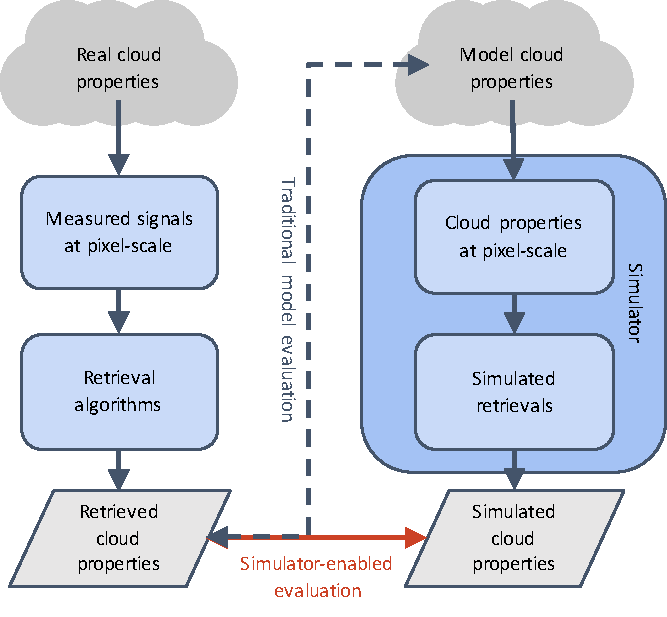
\includegraphics{graphics/simulator_schematic.pdf}
\caption{\label{fig:simulator_schematic}Schematic of the simulator
framework}\label{fig:simulatorux5fschematic}
\end{figure}

The first of these steps, inferring subgrid-scale cloud properties, is
necessary because the resolution of typical global models is much
coarser than the scales at which satellite retrievals are performed. As
pointed out by \citet{pincus_et_al_2012}, these bulk statistics at the
gridbox scale imply a distribution of possible retrievals within each
gridbox, each resulting from a different possible combination of
subgrid-scale profiles. This is due to the fact that simple profiles of
averaged quantities at larger scales do not in themselves fully
constrain the distribution of profiles at smaller scales, and simulating
the satellite views of clouds depends on detailed knowledge of the
overlapping nature of clouds and precipitation at scales approximating
satellite pixels. This is accounted for in the simulator framework by
generating stochastic samples of ``subcolumn'' profiles, which reproduce
the gridbox-averaged profiles in the limit of many samples and are
consistent with some external assumption about how the cloudy parts of
the gridbox overlap vertically \citep{klein_and_jakob_1999}. This
problem is not unique to simulating satellite-retrieved quantities, but
is also important for simulating radiative fluxes and heating rates
within models as well. In COSP, the assumption is made in the subcolumn
sampling process that cloud occurrence obeys a conceptually simple
combination of maximum and random overlap and that cloud (and
precipitation) condensate is horizontally homogeneous on the scale of
model gridboxes. These same assumptions are often (but not always) used
in models for the simulation of radiative fluxes. It has been shown that
these assumptions can lead to substantial errors in simulated radiative
fluxes and heating rates in models
\citep{barker_et_al_1999, oreopoulos_et_al_2012}, and in Chapter~3 here
it is shown that these assumptions similarly lead to substantial errors
in simulated satellite retrievals. In Chapter~4 an improved framework
for sampling these subcolumns is presented that better represents the
subgrid-scale cloud and precipitation properties, and it is shown that
these improvements can substantially reduce the errors identified in
Chapter~3.

Errors in the second step in the simulator framework (simulating the
pixel-scale satellite retrievals), can arise due to incomplete or
incorrect implementation of the retrieval process, even given perfect
pixel-scale cloud properties as inputs. While every effort is made to
build the simulators to account for as many features of the individual
retrievals as possible, verification of the simulators is difficult, and
documented verification is limited in the literature. The basic question
that largely remains unanswered is, given perfect descriptions of the
cloudy atmosphere as inputs to the simulators, are they able to
faithfully reproduce the retrieved cloud properties that the instrument
they attempt to simulate actually retrieves? A theoretical framework for
answering this question is to supply ``observed profiles'' of cloud
properties as inputs to the simulators, and then to compare the
simulated retrievals with coincident retrievals. Using this framework to
answer this question is difficult because it requires some source for
these ``observed profiles''. \citet{mace_et_al_2009} and
\citet{mace_et_al_2011} use a multi-sensor approach combining
ground-based remote sensing retrievals of cloud properties to derive
inputs to the ISCCP simulator, run the ISCCP simulator directly on these
inputs and then compare the simulated ISCCP cloud properties with actual
coincident ISCCP retrievals. While the input profiles derived from the
ground-based retrievals are likely imperfect and have their own
associated uncertainties (which must be considered in the analysis),
studies such as these are important for building confidence in the
fidelity of the simulator framework itself. In Chapter~2, an evaluation
of the MISR simulator is presented, using a conceptually similar
framework to that used in \citet{mace_et_al_2009} and
\citet{mace_et_al_2011}.
